
\chapter{Results}

From the process outlined above, 787,058 galaxy pairs were constructed with a mean angular separation of $\sim 27.6 $ arcmins, and a mean comoving separation of $11.9 h^{-1}$ Mpc. 

\begin{figure}[H]
\centering
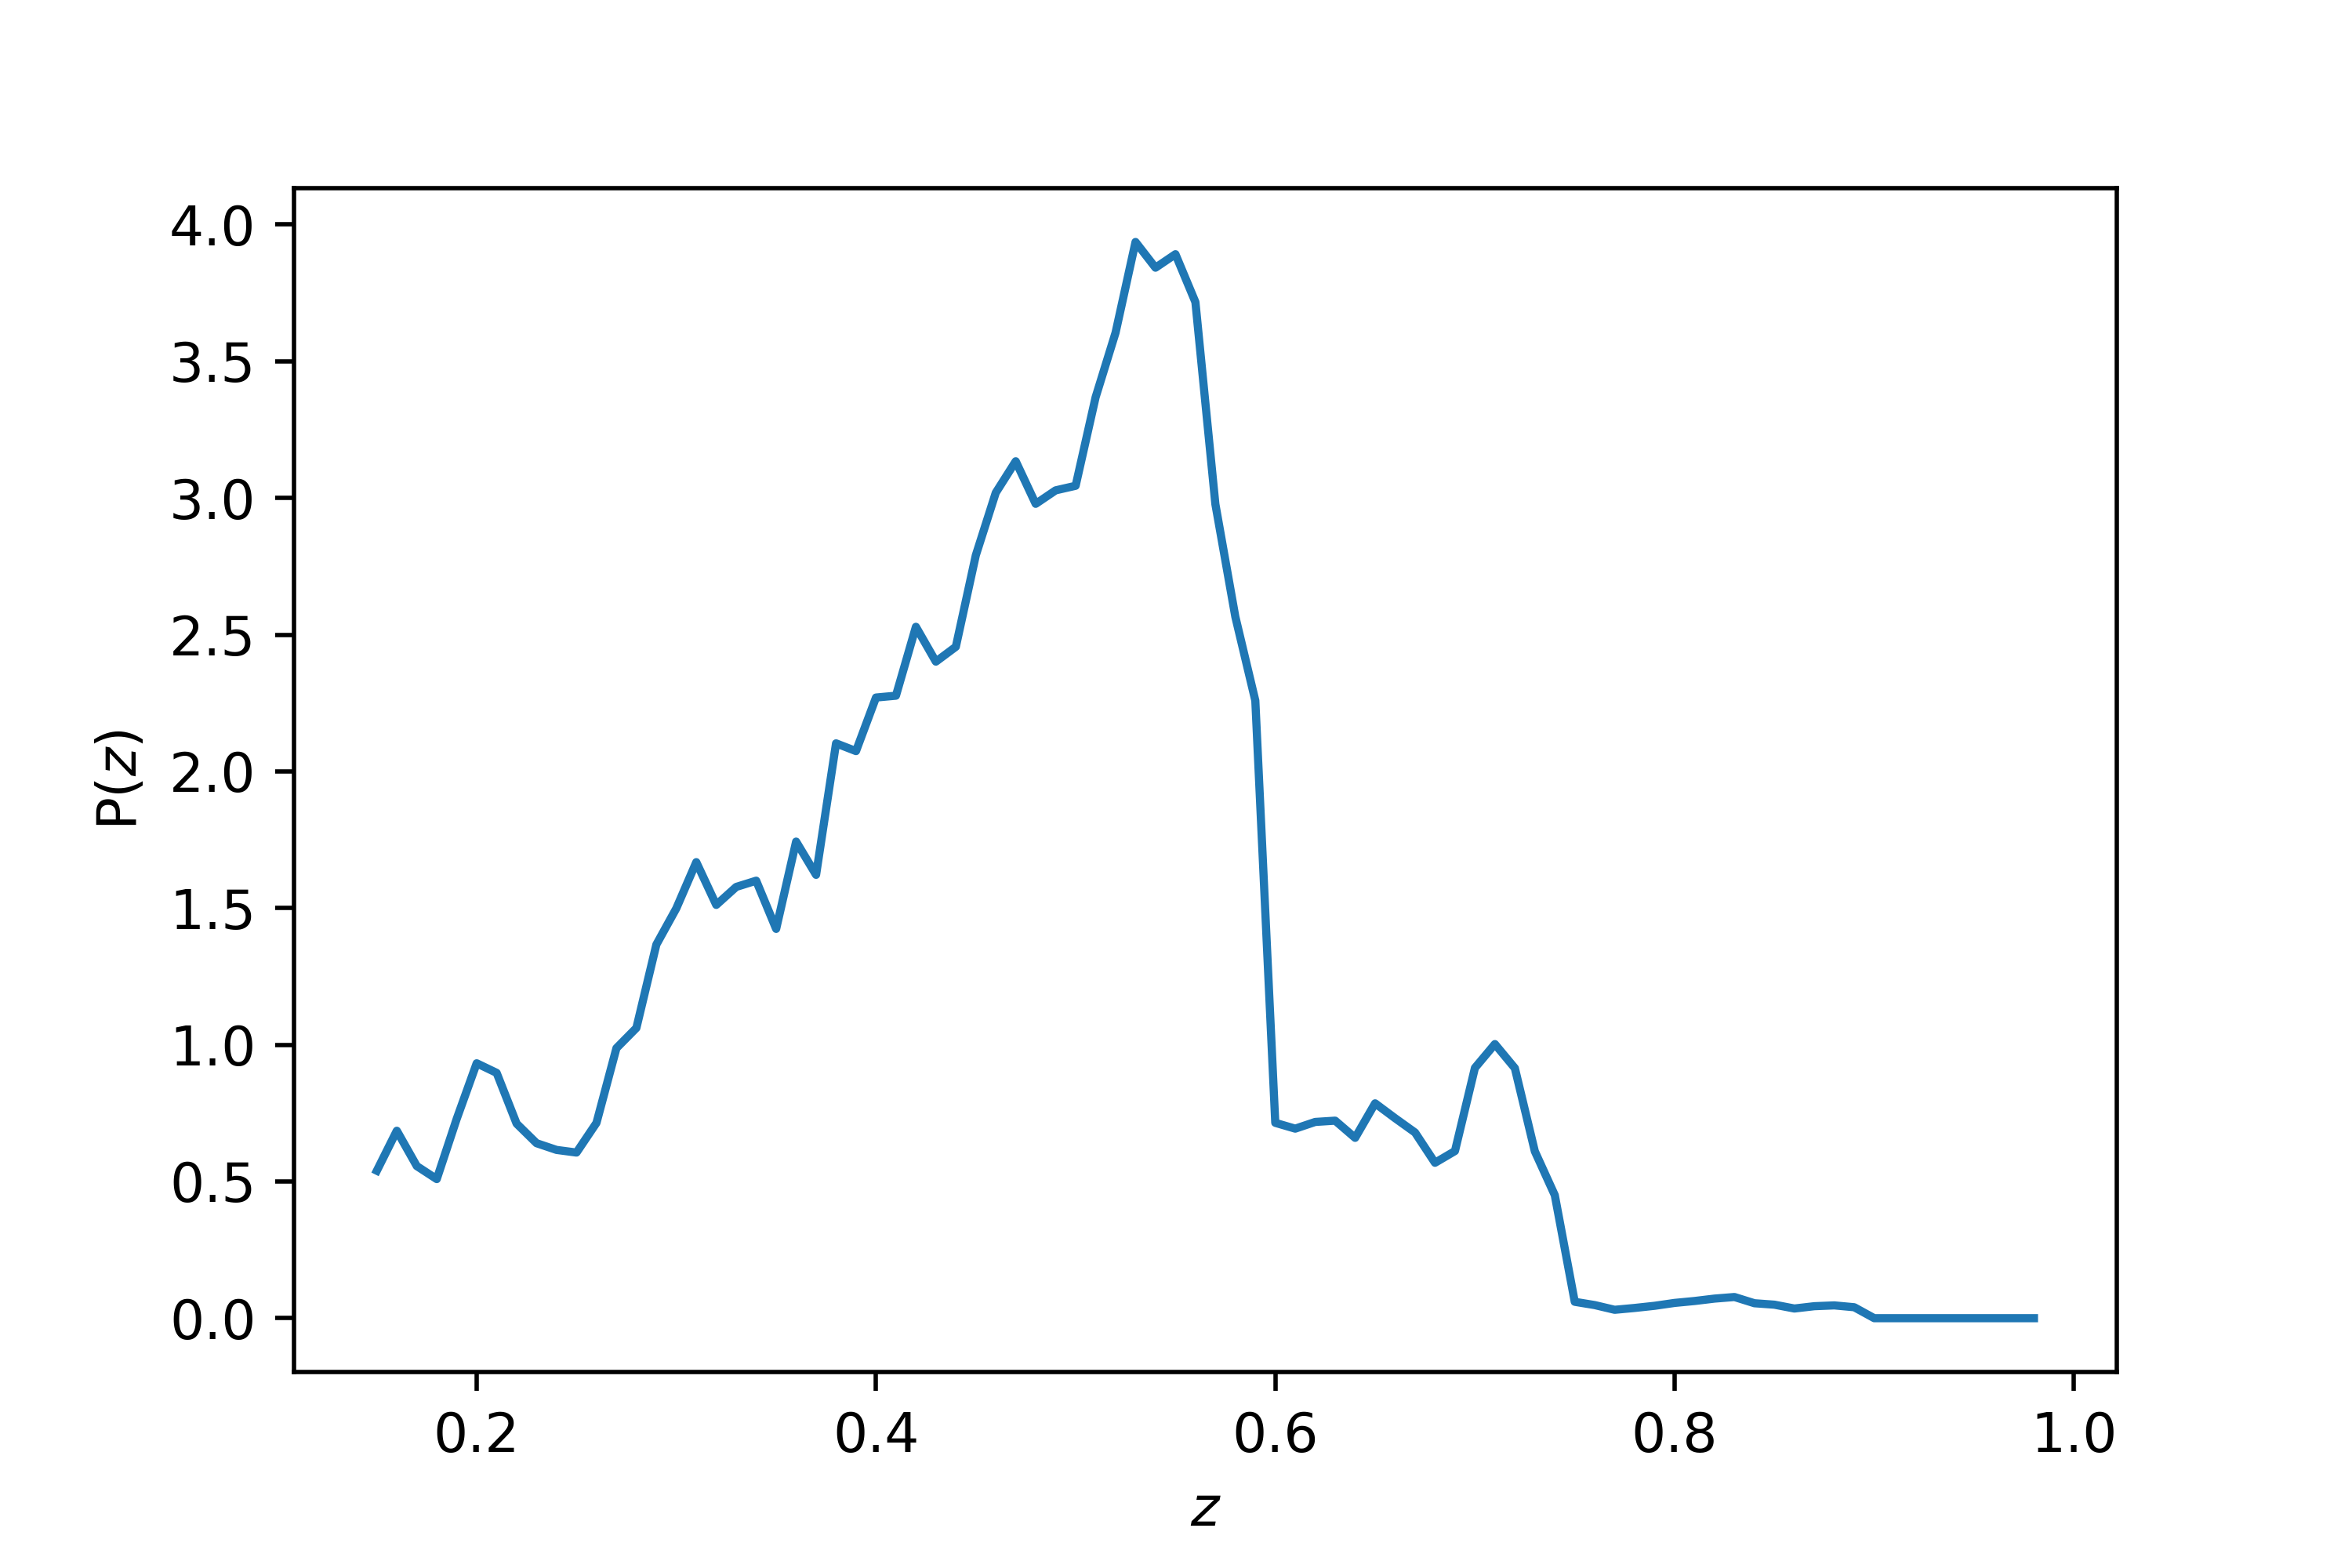
\includegraphics[width=0.6\textwidth , keepaspectratio]{/home/mitchell/Documents/masters/masters/thesis/Ver_2/figures/Redshift_Distribution.png}
\caption{Redshift Distributions of Physical Pairs. The pairs range from redshifts $z\approx0.15$ to $z\approx0.90$, with a mean redshift of $z\approx0.50$.}
\label{fig:physical:redshifts}
\end{figure}

Figure \ref{fig:physical:redshifts} shows the overall PDF of galaxy pairs as a function of redshift. It shows that the mean redshift for the pairs is $z=0.468$, with a minimum redshift of $z= 0.15$, and a maximum redshift of $z= 0.90$. There is a rather drastic drop in the galaxy population after redshift $z \sim 0.58$. This is due to there being fewer galaxies in the higher redshift bins in the DES Year 1 Catalogue. Figures \ref{fig:physical:lineofsight} and \ref{fig:physical:transverse} show the line-of-sight and transverse separation PDFs of the pairs.

\begin{figure}[H]
\centering
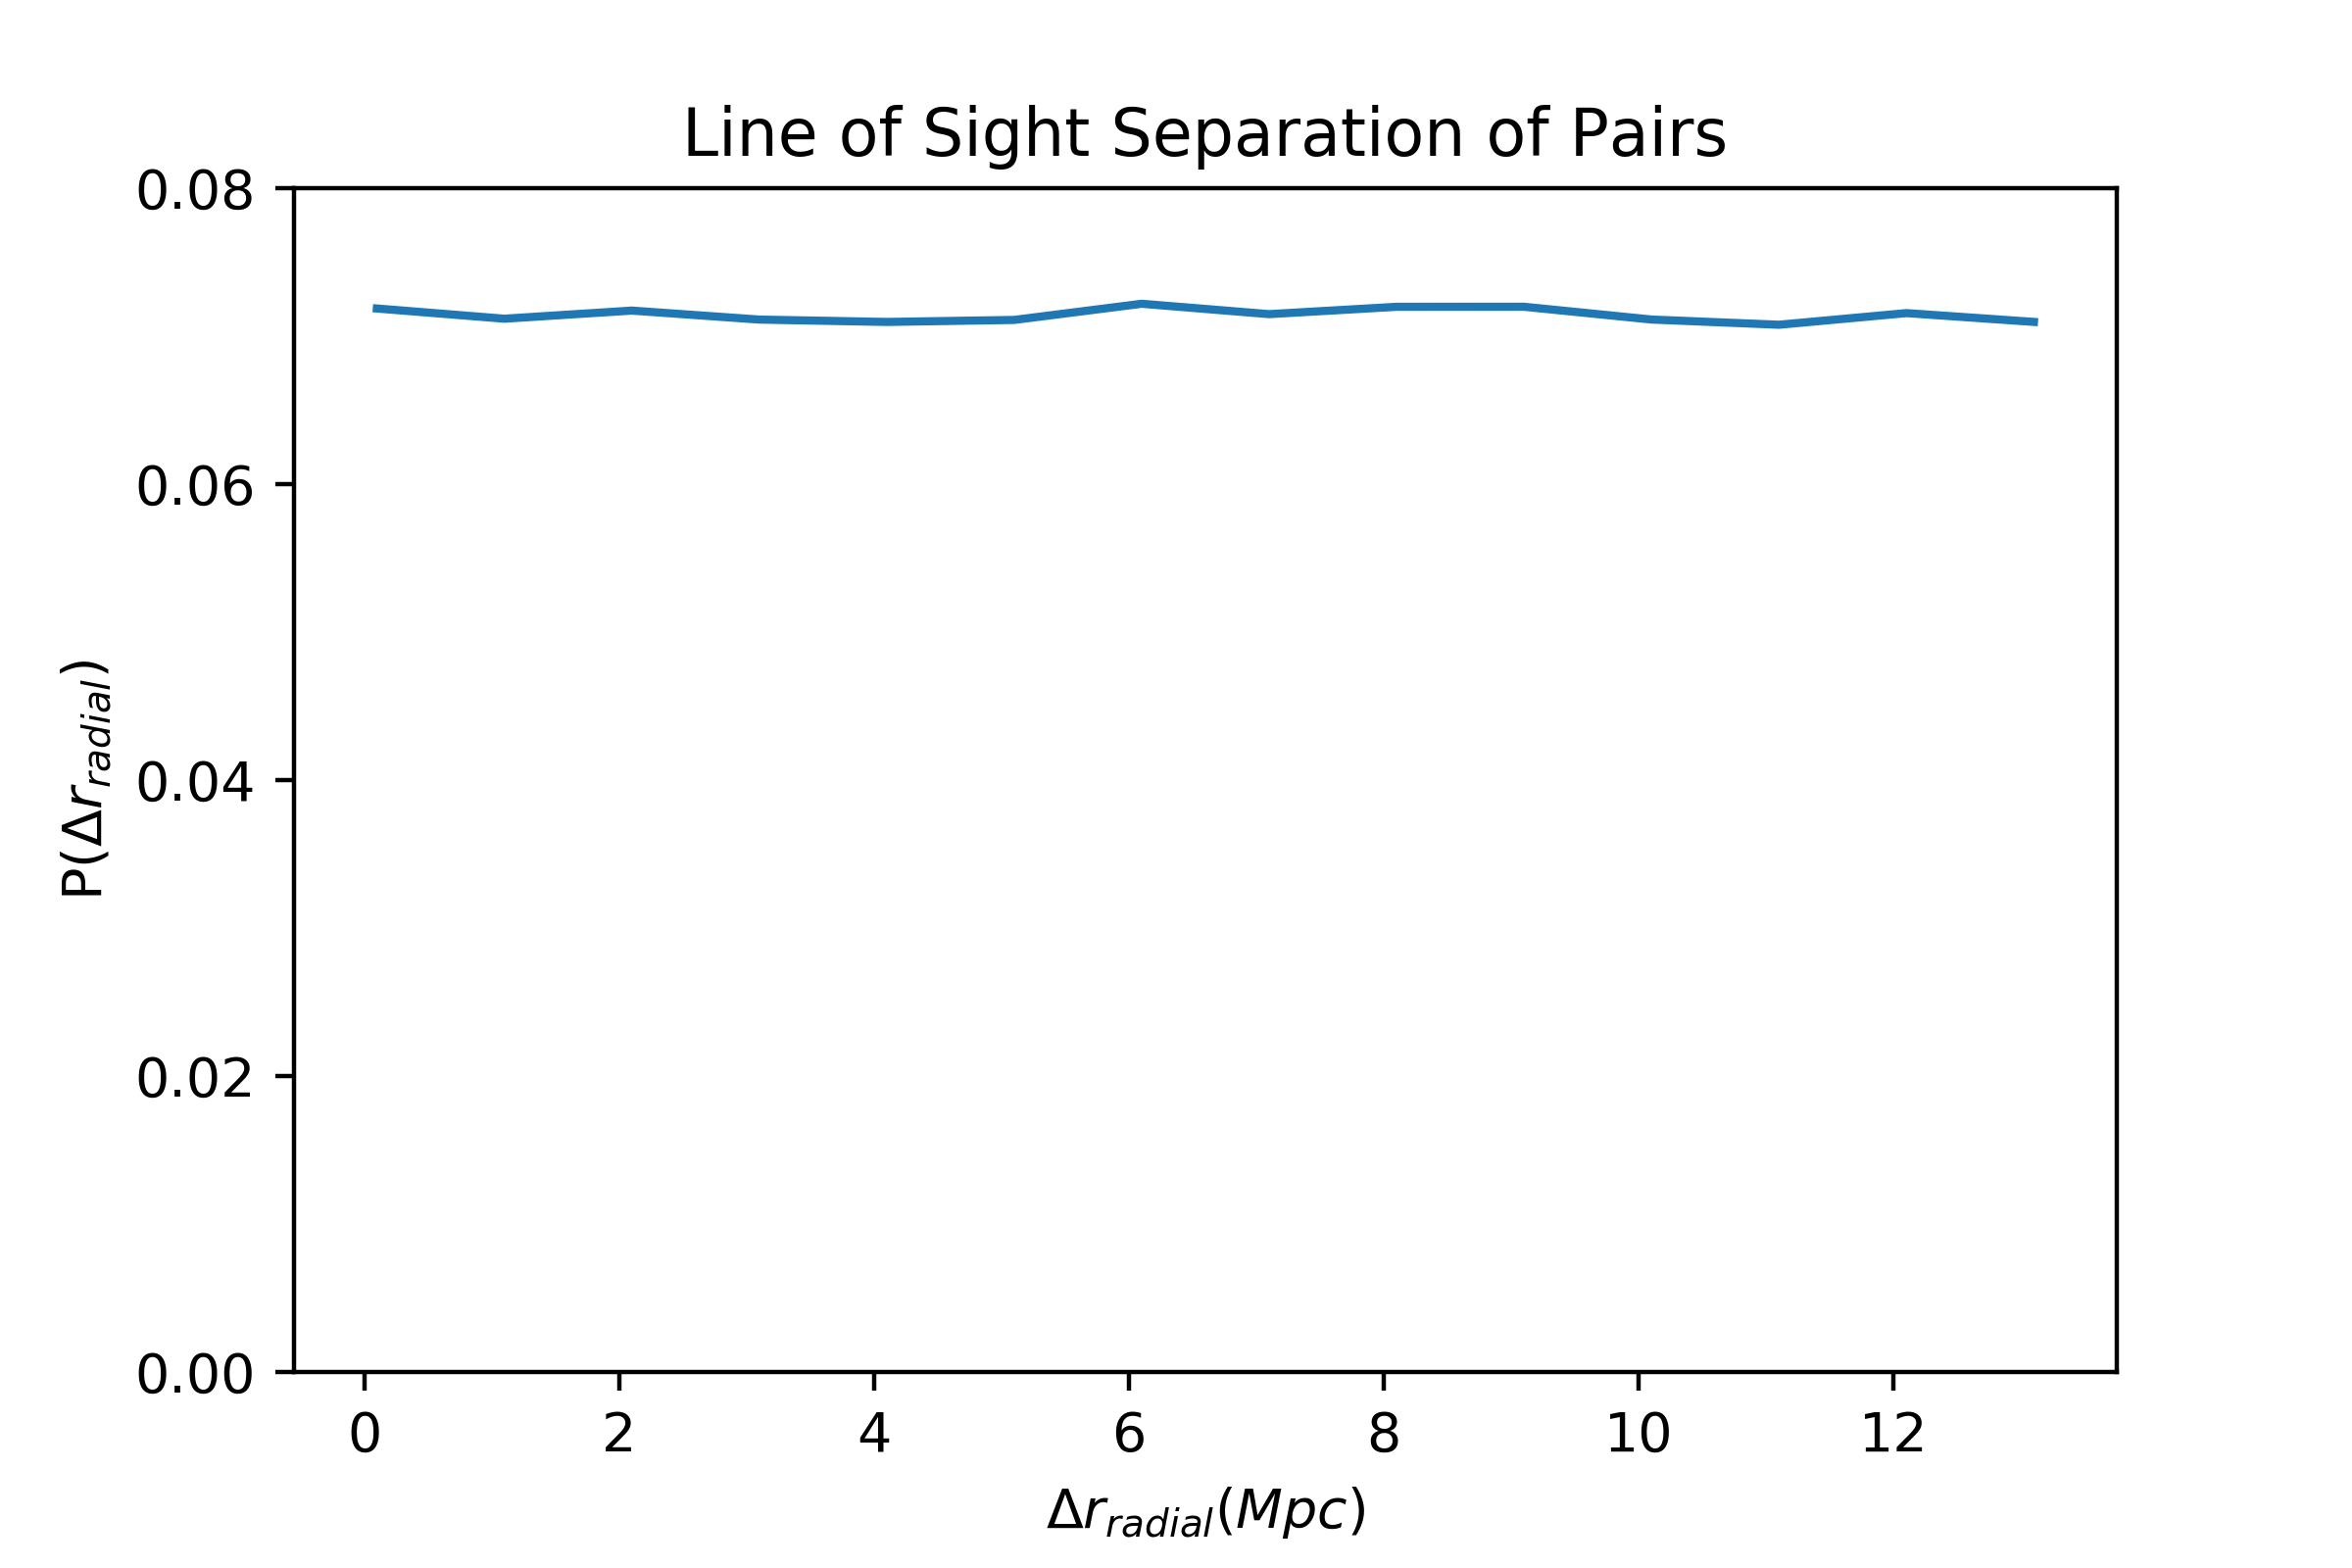
\includegraphics[width=0.6\textwidth , keepaspectratio]{/home/mitchell/Documents/masters/masters/thesis/Ver_2/figures/LOS_Separation.png}
\caption{Histogram of Line of Sight Separations of Galaxy Pairs. The distribution is relatively flat, with a minimum separation of $\SI{0}{\mega\parsec}$, and a maximum separation of $\SI{14.8}{\mega\parsec}$.}
\label{fig:physical:lineofsight}
\end{figure}


\begin{figure}[H]
\centering
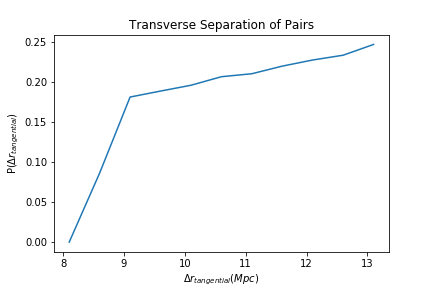
\includegraphics[width=0.6\textwidth , keepaspectratio]{/home/mitchell/Documents/masters/masters/thesis/Ver_2/figures/TRV_Separation.png}
\caption{Histogram of Transverse Separations of Galaxy Pairs. The distribution climbs steadily, with a minimum seperation of $\SI{8.85}{\mega\parsec}$ and a maximum separation $\SI{20.7}{\mega\parsec}$. }
\label{fig:physical:transverse}
\end{figure}

\par There are more pairs in higher transverse separation bins than in lower ones, which suggests that there will be a tendency to rescale pairs by smaller amounts in the algorithm. This will also effect the resulting halo shape, since pairs that are closer together will also by nature be scaled to larger effective halo sizes.  

The stacking procedure was performed on a Compton $y$-map produced from a combination of the South Pole Telescope SZ observing run, and the \emph{Planck} datasets. It made use of the $\SI{90}{\giga\hertz}$, $\SI{150}{\giga\hertz}$, and $\SI{220}{\giga\hertz}$ maps from SPT-SZ, and combined them with the $\SI{100}{\giga\hertz} - \SI{350}{\giga\hertz}$ and dust maps from \emph{Planck}, in the same manner as is described in \cite{2016ApJS..227...23C} (Bleem, in prep.). The algorithm for producing this map also took the half survey and half mission power spectra from \emph{Planck} as inputs. It minimised the contribution of the primary CMB, Cosmic Infrared Background (CIB), Instrumental, and Atmospheric sources as the primary sources of noise. 

We performed the stack on a map with a resolution of $\SI{0.25}{\arcmin}$ per pixel, but the effective resolution, after combining the beam sizes of the various raw data maps, is closer to $\SI{2}{arcmin}$, so there is likely some interpolation in the output, which would have introduced a source of noise.


Stacking these pairs returns an average $y$ map, which is shown in figure \ref{fig:physical:stack}. The signal is dominated by the contribution of the galaxy halos, and so these will need to be effectively subtracted in order to evaluate the significance of the filament signal. To the eye, there appears to be some residual signal in between the two halos, which has not been driven to zero as a result of the stacking process. 


\begin{figure}[H]
\centering
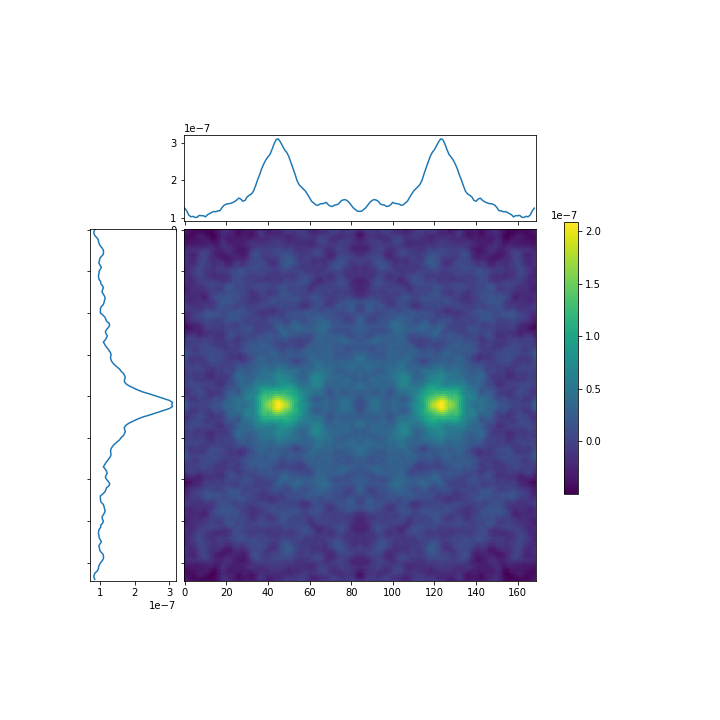
\includegraphics[width=\textwidth , keepaspectratio]{/home/mitchell/Documents/masters/masters/thesis/Ver_2/figures/Stack.png}
\caption{Stacked Image of galaxy pairs. The upper panel shows the slice through the centre of the stack. The left panel displays a vertical slice through the left halo, which by the mirroring procedurce, will be the same as the slice through the right halo.}
\label{fig:physical:stack}
\end{figure}

Once we have stacked the pairs, we perform our fit, as described in \ref{alg:analysis}. Beginning with our naive fit, we considered only a single halo, because the mirroring of the image essentially forces the two halos to look identical under this calculation. We also only consider the half of the halo that is on the other side to the filament, to prevent contamination from the filament. Doing so yields a halo shape shown in Figure \ref{fig:halo:single}.

\begin{figure}[H]
\centering
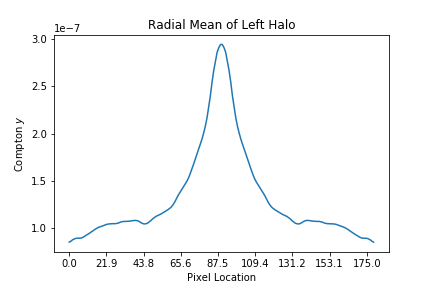
\includegraphics[width=\textwidth , keepaspectratio]{/home/mitchell/Documents/masters/masters/thesis/Ver_2/figures/halo_shape.png}
\caption{ Radial Mean of Left Halo from figure \ref{fig:physical:stack}. The shape of the halo does not appear to be gaussian in nature, perhaps owing to the uneven scaling depending on transverse separations. }
\label{fig:halo:single}
\end{figure}

Taking this halo shape, and assuming that there is some constant background signal of approximately $y = 1\times 10^{-7}$, we can combine this into our naive model, and find a measure of the residual filament. Assumig this constant background signal is functionally the same as taking a high bandpass filter of the stack. 


\begin{figure}[H]
\centering
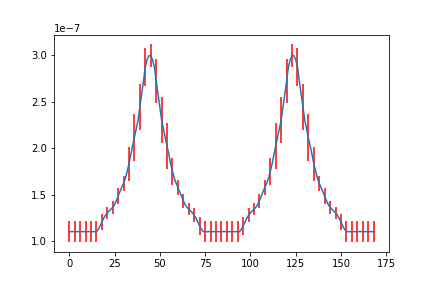
\includegraphics[width=\textwidth , keepaspectratio]{/home/mitchell/Documents/masters/masters/thesis/Ver_2/figures/halo_model_basic.png}
\caption{ Basic Halo Model, constructed from the radial mean of a single halo, with error bars given by the standard deviation of the halo in the same radial bins }
\label{fig:halo:basic_model}
\end{figure}

Figure \ref{fig:halo:basic_model} shows this model, with errors derived from computing the standard deviation of the radial halo in the same halo bins as the mean was calculated. Subtracting this from the slice through the halos gives us the graph shown in figure \ref{fig:halo:basic_filament}.

\begin{figure}[H]
\centering
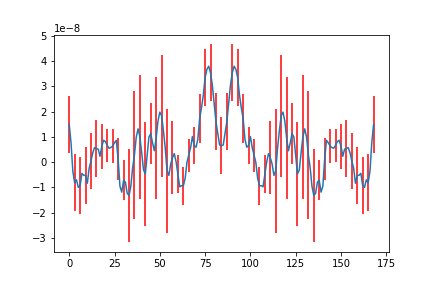
\includegraphics[width=\textwidth , keepaspectratio]{/home/mitchell/Documents/masters/masters/thesis/Ver_2/figures/filament_basic.png}
\caption{ Basic Filament Model, with filamentary residual shown between Pixel locations 60 and 110. }
\label{fig:halo:basic_filament}
\end{figure}

This naive calculation shows what is visible to the eye when looking at the stack in figure \ref{fig:physical:stack}, that there is some residual signal in between the two halos which should be from the filaments that connect the galaxy halos. The mean compton y parameter for this region is $\bar{y} \approx 1.9 \times 10^{-8}$, with a mean error of $8.31 \times 10^{-9}$. 



\par If we consider our more complex models in 1 dimension (along the central slice through both halos), and fit to our data, we get the results shown in figure \ref{fig:halo:complex_model}. All models were fit using standard definitions, and using a damped least-squares method known as the Levenberg-Marquardt algorithm.

\begin{figure}[H]
\centering
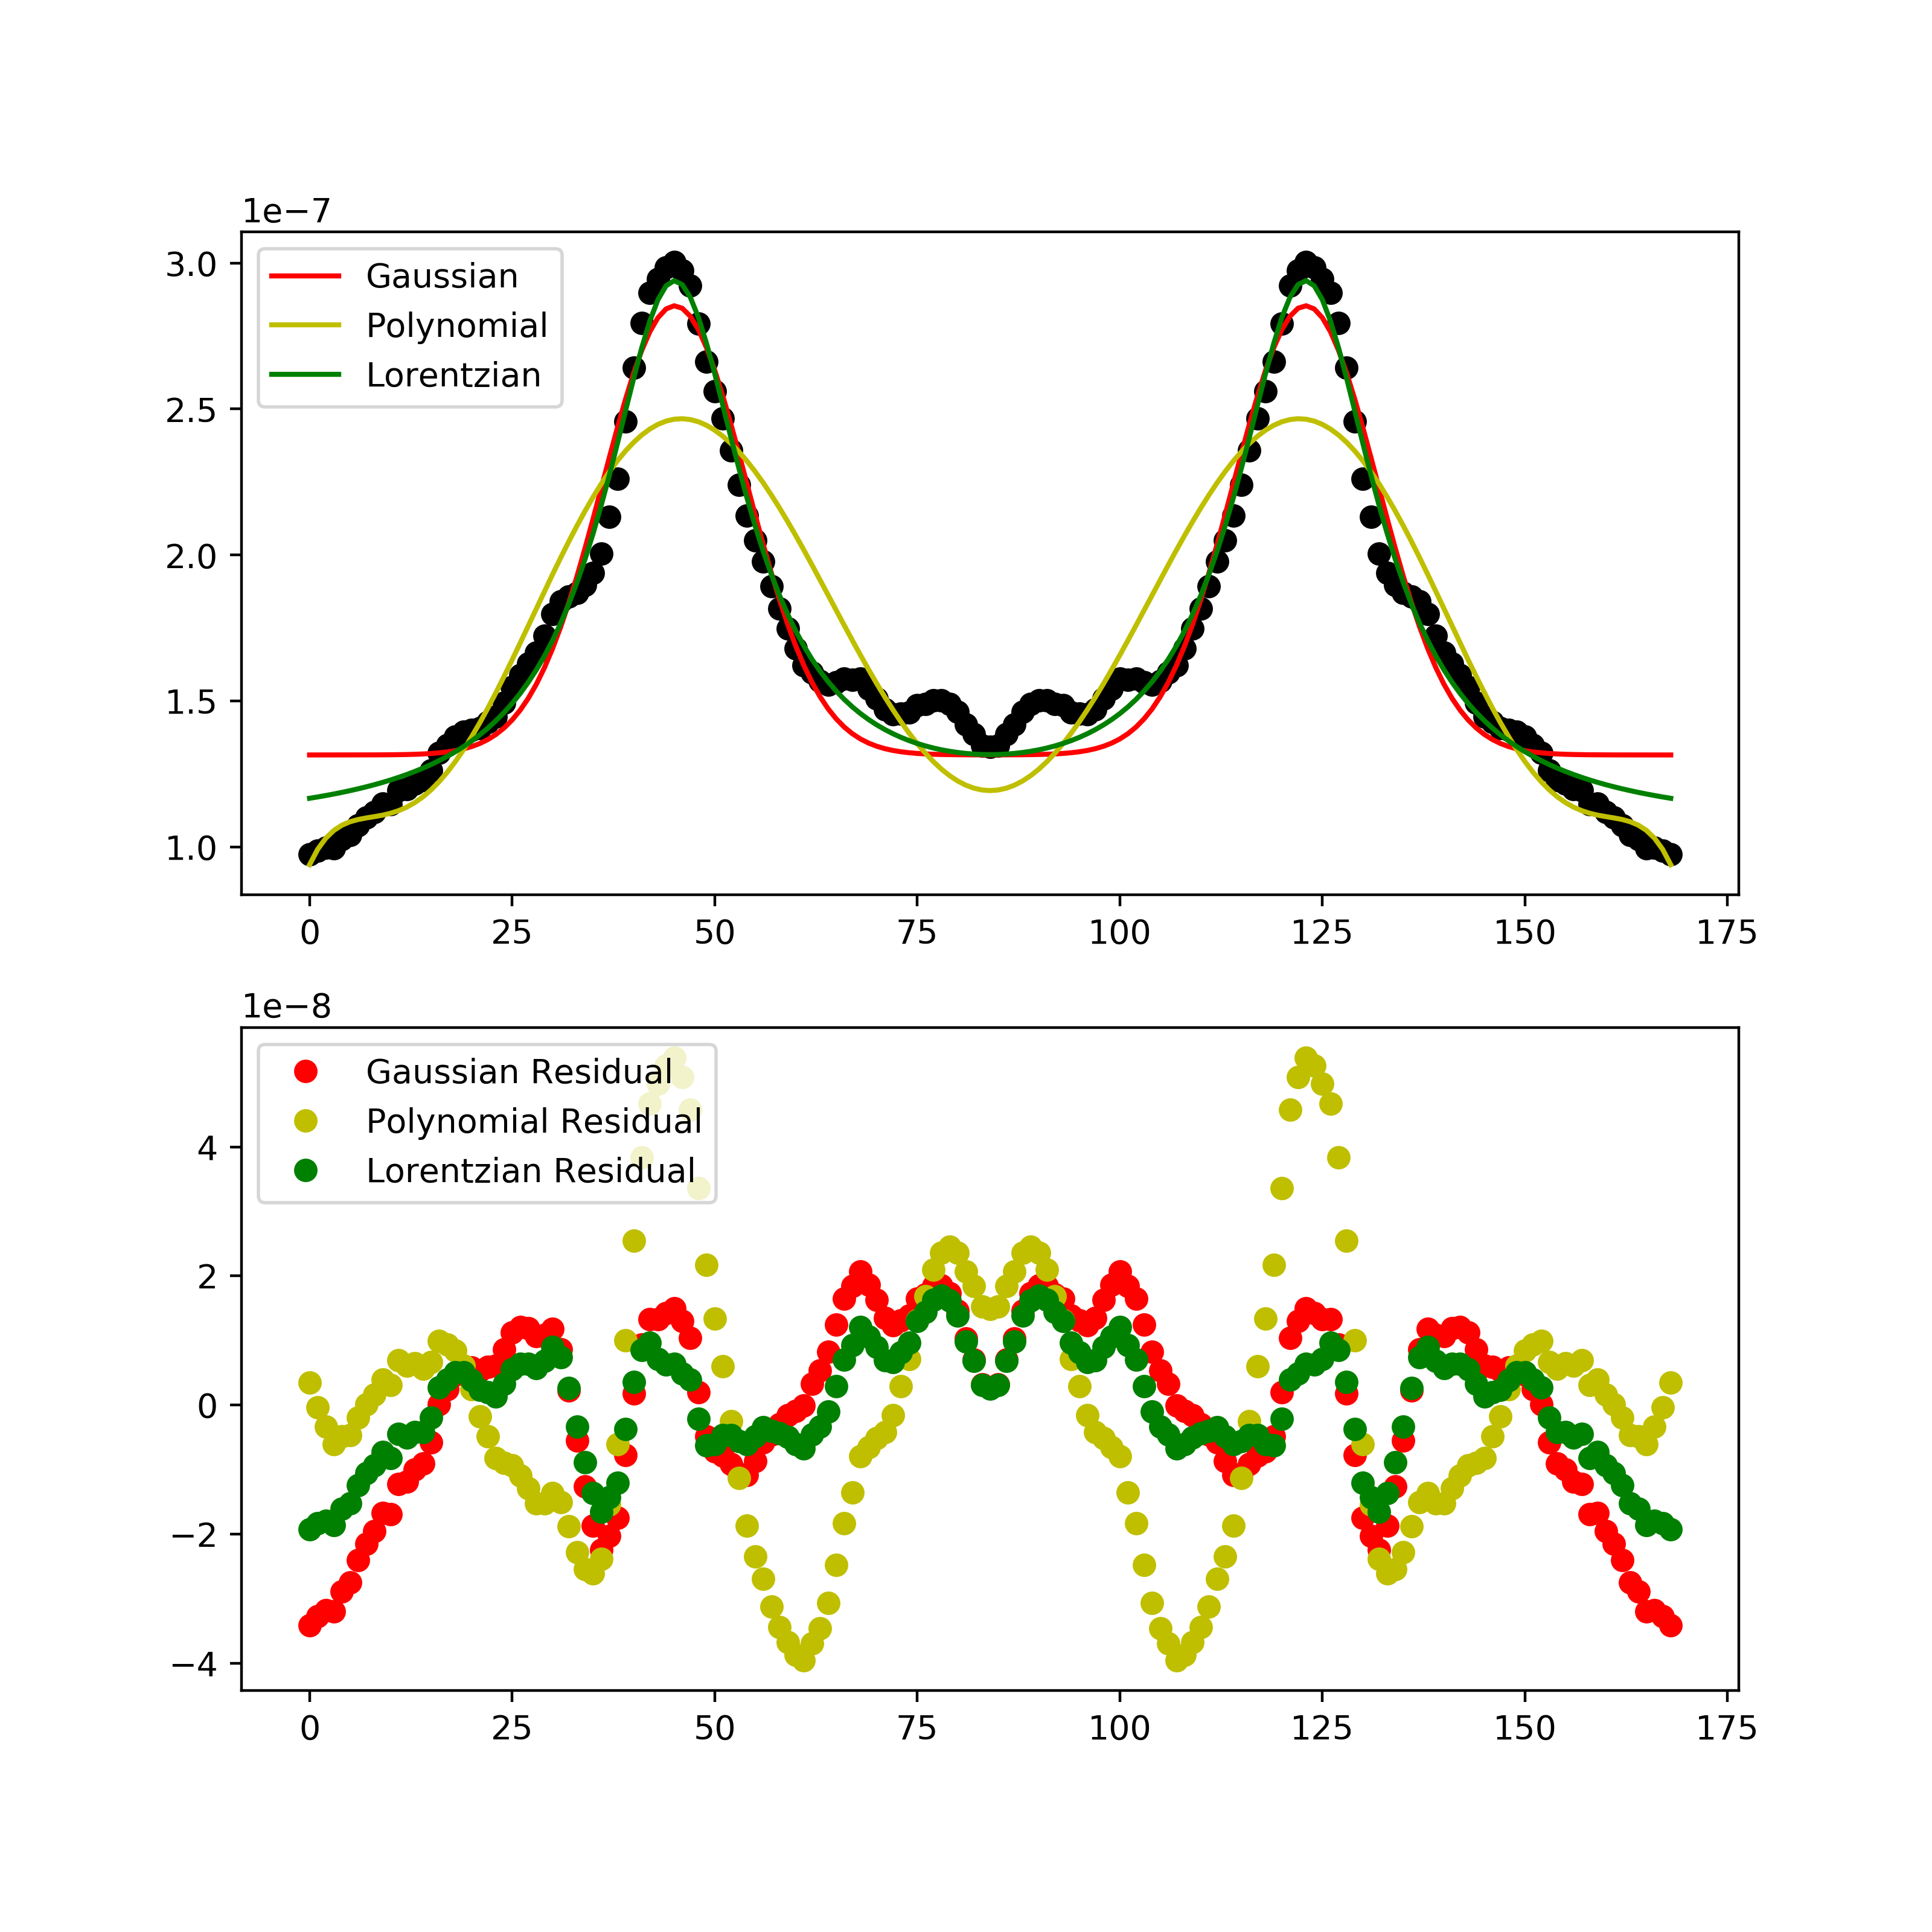
\includegraphics[width=\textwidth , keepaspectratio]{/home/mitchell/Documents/masters/masters/thesis/Ver_2/figures/halo_model_complex.png}
\caption{ Multiple Halo Models fitted to Central Slice of Figure \ref{fig:physical:stack} }
\label{fig:halo:complex_model}
\end{figure}

These are noticably worse than our simple model. The polynomial fit doesn't subtract the halos properly, so we discard it here. The gaussian model does subtract most of the halos away, but the left-over signal is significantly lower, with a mean residual Compton $y$ of $\tilde{y} \approx 8.68 \times 10^{-9}$. The fact that the gaussian models fail to match the curves at the centres of the halos does suggest that it is a poor model.

\par Given the apparent shape was non-gaussian, we applied a Lorentzian fit to the shape of the halos. This fit the halo shapes much better, and dies away much quicker than the gaussian model, but also removes more of the signal we are looking for. It is possibly that this is simply the best fit for the algorithm we have implemented, and a change in our process would result in another model fitting better. It is also incredibly difficult to explain why the halo shape would be lorentzian physically, further reinforcing the idea that it is the result of introduced scaling effects in the algorithm. 

\par Considering that the model of the halo seems to have a non-gaussianity to it, we performed a number of two dimensional model fits to our two dimensional image of the stacks. The models we chose to fit to the data were 
\begin{enumerate}[label=(\Roman*)]
\item 4 Independent Gaussians \label{2D:model:1}
\item 2 sets of 2 coupled Gaussians \label{2D:model:2}
\item 4th order polynomial \label{2D:model:3}
\item Spherical Gaussians \label{2D:model:4}
\end{enumerate}

We chose to use variations of multiple gaussians in order to take into account the distorted shape of the halos. In model \ref{2D:model:1}, we allow 4 gaussians to vary independantly. In model \ref{2D:model:2}, we couple the underlying gaussians together, so that one pair of them will extract the spread of the halo, and another will extract the height. We chose model \ref{2D:model:3} to maintain consistency with our fit from the simple 1D case. In model \ref{2D:model:4}, we force the gaussians to contain our assumption of spherical halos. 

\begin{figure}[H]
\centering
\includegraphics[width=\textwidth , height=\textheight , keepaspectratio]{/home/mitchell/Documents/masters/masters/thesis/Ver_2/figures/2D_data_fitting.png}
\caption{ Multiple Halo Models fitted to 2D array of Figure \ref{fig:physical:stack} }
\label{fig:halo:2D_complex_model}
\end{figure}

When we look at these models, none of them seem to appropriately subtract the halo contributions. 
\par Model \ref{2D:model:1} appears to do the best, removing the majority of the halo, and leaving behind a reasonably strong signal where we would expect to see a filament. What is noticable however, is that the right halo in the model is distorted along some diagonal axis, which is strange, given the data that is being fitted to has been made symmetric about two axes. This results in greater subtraction in the residual of the right halo than the left, and so introduces some error in our measurement of the filament. It also leaves a very large amount of signal in the central region, in what looks like a hourglass shape. It is unclear if this is indicative that filaments don't necessarily link galaxies in a straight line, or if it is an artefact of the mirroring process.
\par If we correct for the perceived issues with the first model, model \ref{2D:model:2} forces the gaussians into sets of two, which each obey the same statistics, therefore accounting for the mirroring in the image. This form of the model does succeed in extracting nearly all of the halo, but leaves so much residual signal everywhere that it looks like we are extracting residual baryons from areas surrounding the galactic halos. 

\par Unfortunately, \ref{2D:model:3} extracts too much of the signal, and not enough of the halos. This may be due to the way that the model is being fit to the data. Since the data is symmetric about the central $x$ axis, the model fitting will see the same value on both sides of the masked area. This forces the fit to assume that the data holds the same value across the masked area, removing the possibility that the halos fall away, and so preventing us from detecting the filament signal. If we perform the fit on the whole array of data, the polynomial overfits the data, and subtracts the entirety of the filament signal anyway. The current fit doesn't subtract the whole halo signal either, meaning that the data isn't being fit properly with the current mask. 
\par Model \ref{2D:model:4} also extracts too much of the filament signal. It appears that forcing the spherical shape of the halos causes too much crossover in the modelled halos. This effectively leaves us with no filament signal, allowing us to discard this model. Doing so does raise some interesting points however, regarding our assumption of spherical symmetry. 


\par These two dimensional models do not perform as well as the one dimensional ones, either in terms of accuracy or strength of signal. This is likely due to the increased amount of noise in the two dimensional image, as opposed to the one dimensional slice. The higher resolution in the $y$ map we use could also be introducing this higher level of noise, since it would not necessarily be smoothed out by the detector beam. 

\par The results for all models which are considered sensible are included in Table \ref{table:results}. 

\begin{table}[H]
\centering
\begin{tabular}{||c c c c||} 
 \hline
 Model & Mean Residual $y$  & Error & Sigma\\
 \hline\hline
 Radial Mean 1D Fit & $2.5\times 10^{-8} $ & $\pm 7.72 \times 10^{-9}$ & $3.24$\\
 \hline
 1D Gaussian Fit & $1.29\times 10^{-8} $ &  $\pm 6.29 \times 10^{-9}$ & $2.05$\\
 \hline
 2D Model 1 & $1.38\times 10^{-8}$ & $\pm 1.77 \times 10^{-8}$ &  - \\
 \hline 
 2D Model 2 & $0.82 \times 10^{-9} $ &  $\pm 1.59 \times 10^{-8}$ & - \\
 \hline \hline 
\end{tabular}
\caption{Results for residual mean filament for various fitting methods }
\label{table:results}
\end{table}

Given the necessity of accounting for both halo contributions at all points in the stack, we hold that the best result to quote is the 1D gaussian fit. Our fiducial value of the average Compton-$y$ of the filament is 
\begin{equation}
\boxed{\bar y = 1.29 \times 10^{-8} \pm 6.29 \times 10^{-9}}
\end{equation}
\section{Null Tests}
\subsection{Un-Physical Pairs}
We constructed a catalogue of unphysical pairs from the galaxies contained in both the SPTpol and DES survey footprints, with radial separations between $\SI{100}{\per\h\mega\parsec}$ and $\SI{200}{\per\h\mega\parsec}$, and transverse separations between $\SI{6}{\per\h\mega\parsec}$ and $\SI{14}{\per\h\mega\parsec}$. 

\begin{figure}[H]
\centering
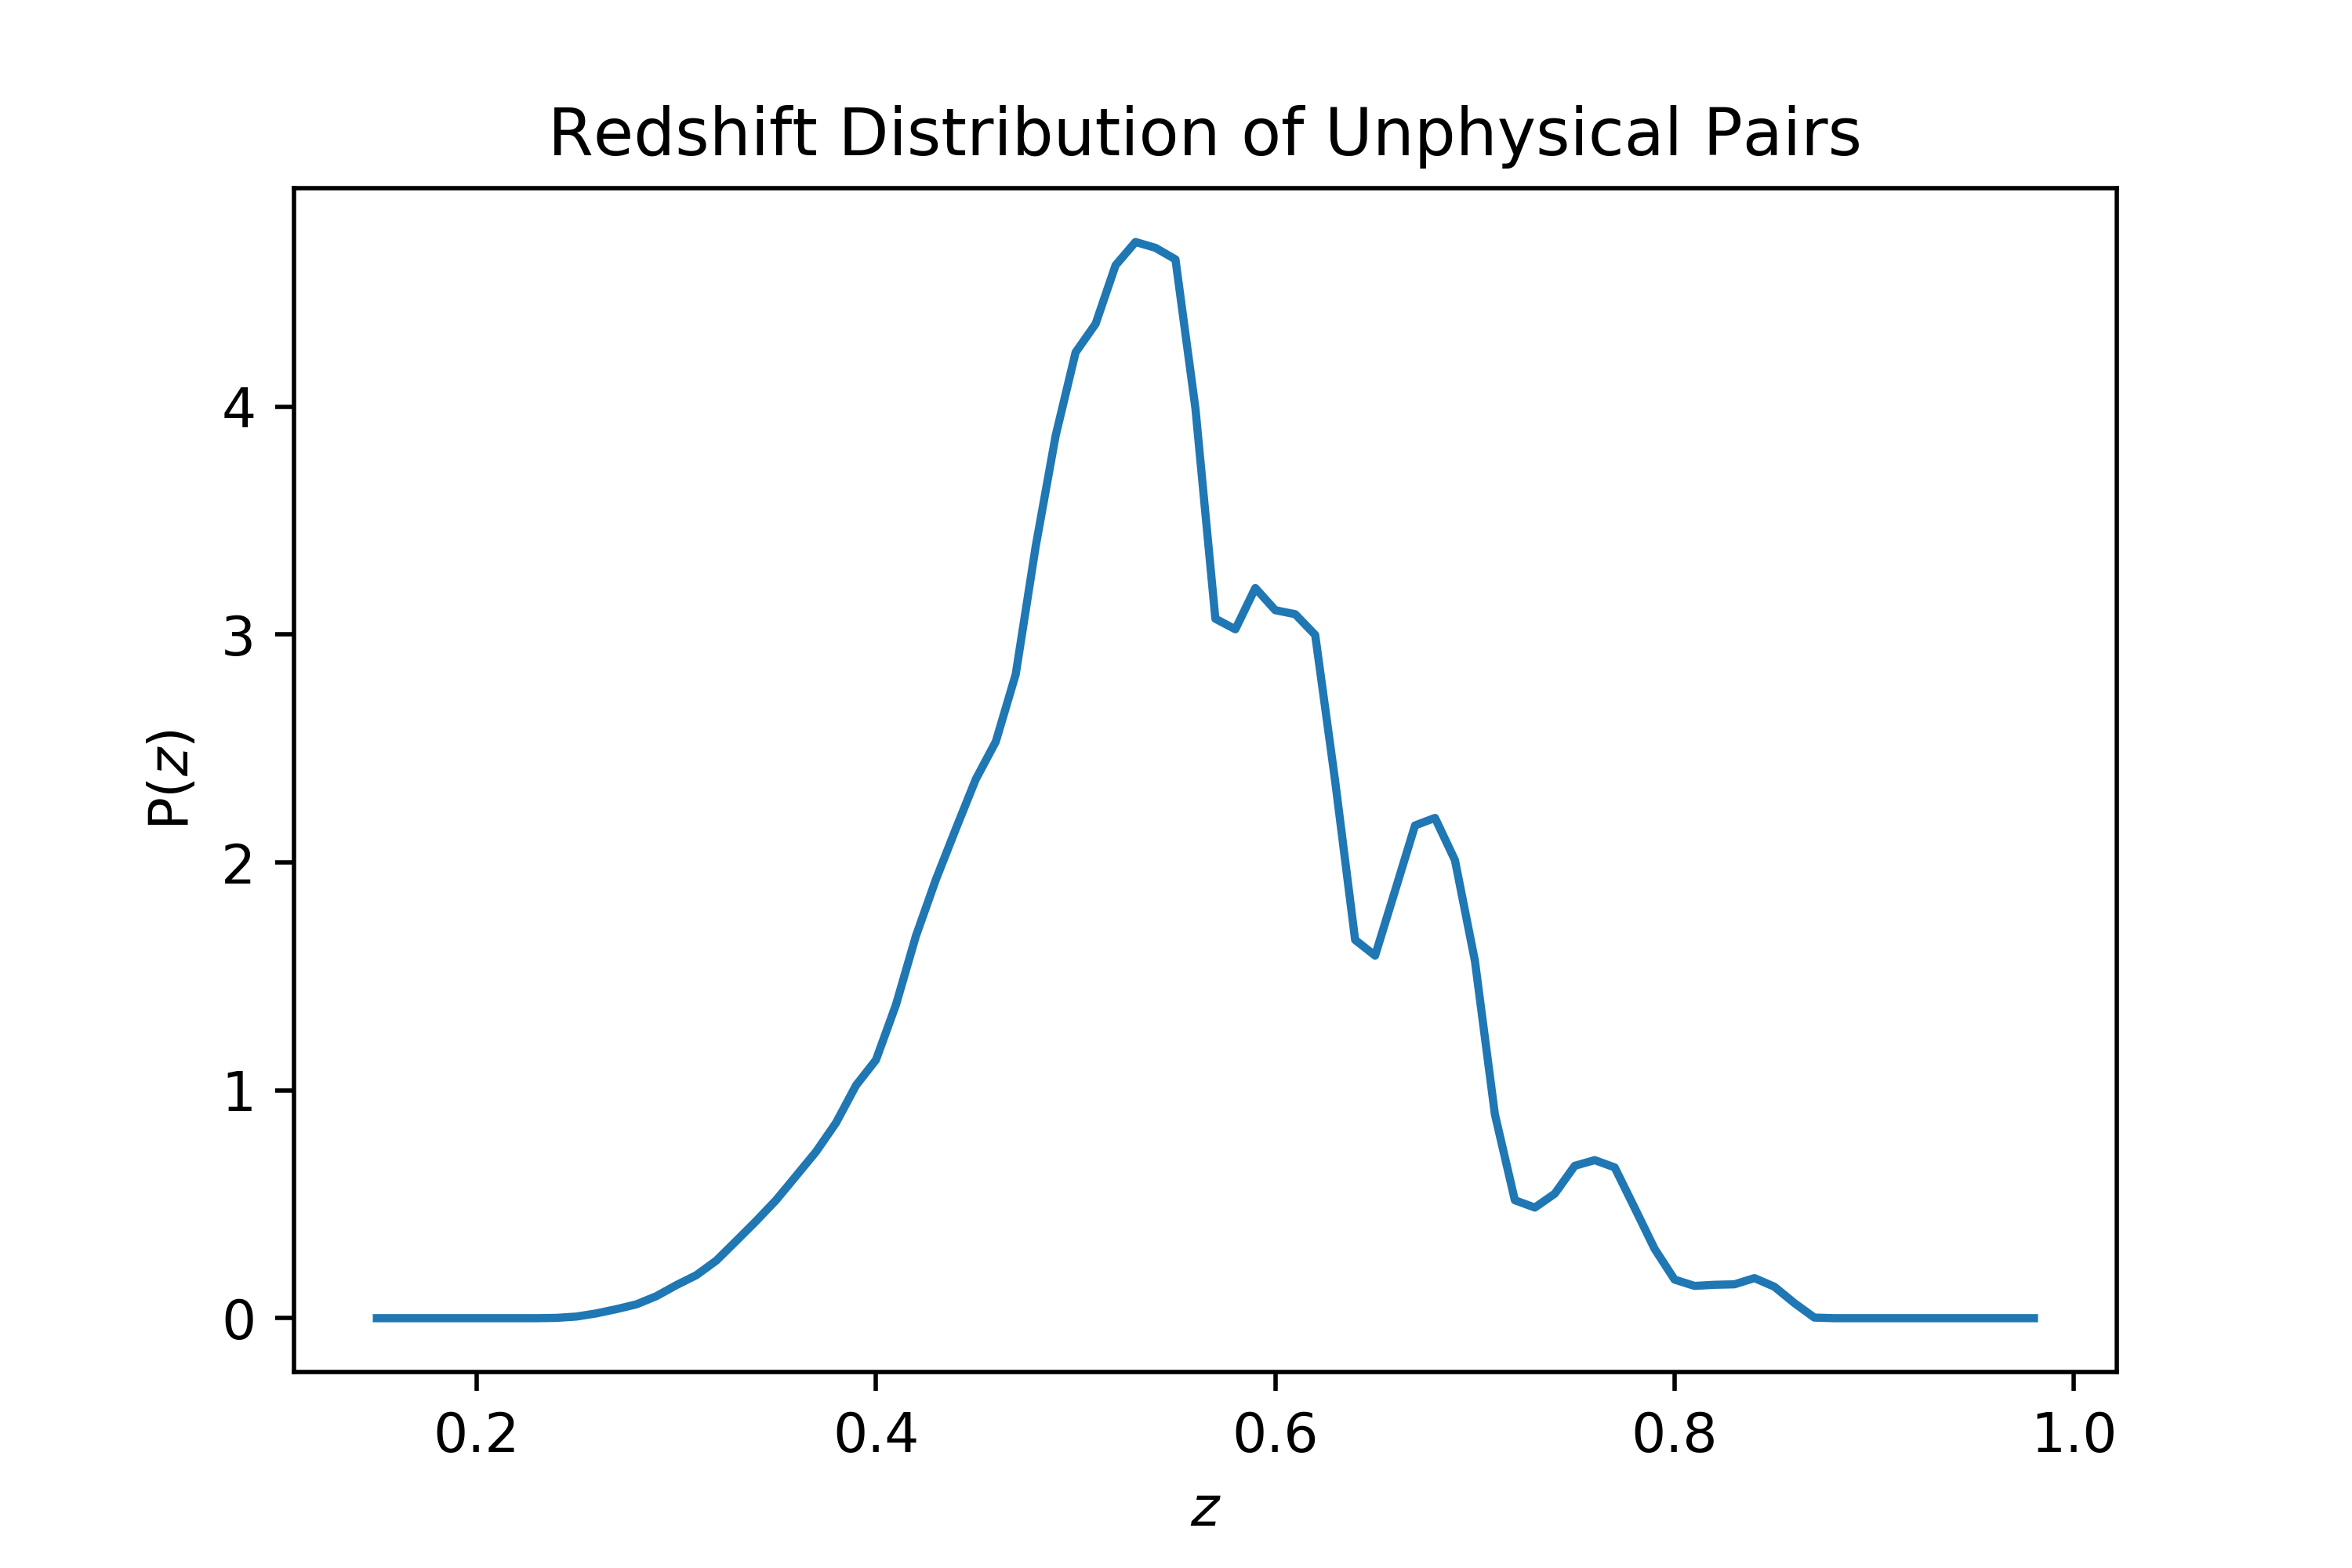
\includegraphics[width=0.6\textwidth , keepaspectratio]{/home/mitchell/Documents/masters/masters/thesis/Ver_2/figures/UnPhysical_Redshift_Distribution.png}
\caption{Redshift Distributions of Unphysical Pairs. The pairs range from redshifts $z\approx0.24$ to $z\approx0.87$, with a mean redshift of $z\approx0.55$. When compared to the physical pairs, this set has a higher mean redshift, and more pairs in higher redshift bins.   . The distribution of physical pairs is overlaid in red.}
\label{fig:unphysical:redshifts}
\end{figure}
As can be seen in figure \ref{fig:unphysical:redshifts}, the distribution of redshifts is generally skewed towards higher redshifts than for the physical pairs. This is likely due to the inherent errors assosciated with the photometric redshifts in the DES redMaGiC survey. Lower redshifts are more likely to be more precise, since the photometric errors for redshift are given by $\Delta z= 0.01(1+z)$, and so be excluded by the line of sight cuts. The other effect which may influence this is the fact that there are far more pairs in the unphysical dataset than in the physical dataset. 


This produced a set of unphysical pairs containing $\sim 670,000$ pairs, with a mean line of sigh separation of $\SI{220}{\mega\parsec}$, and a mean transverse separation of $\SI{12.5}{\mega\parsec}$.


\begin{figure}[H]
\centering
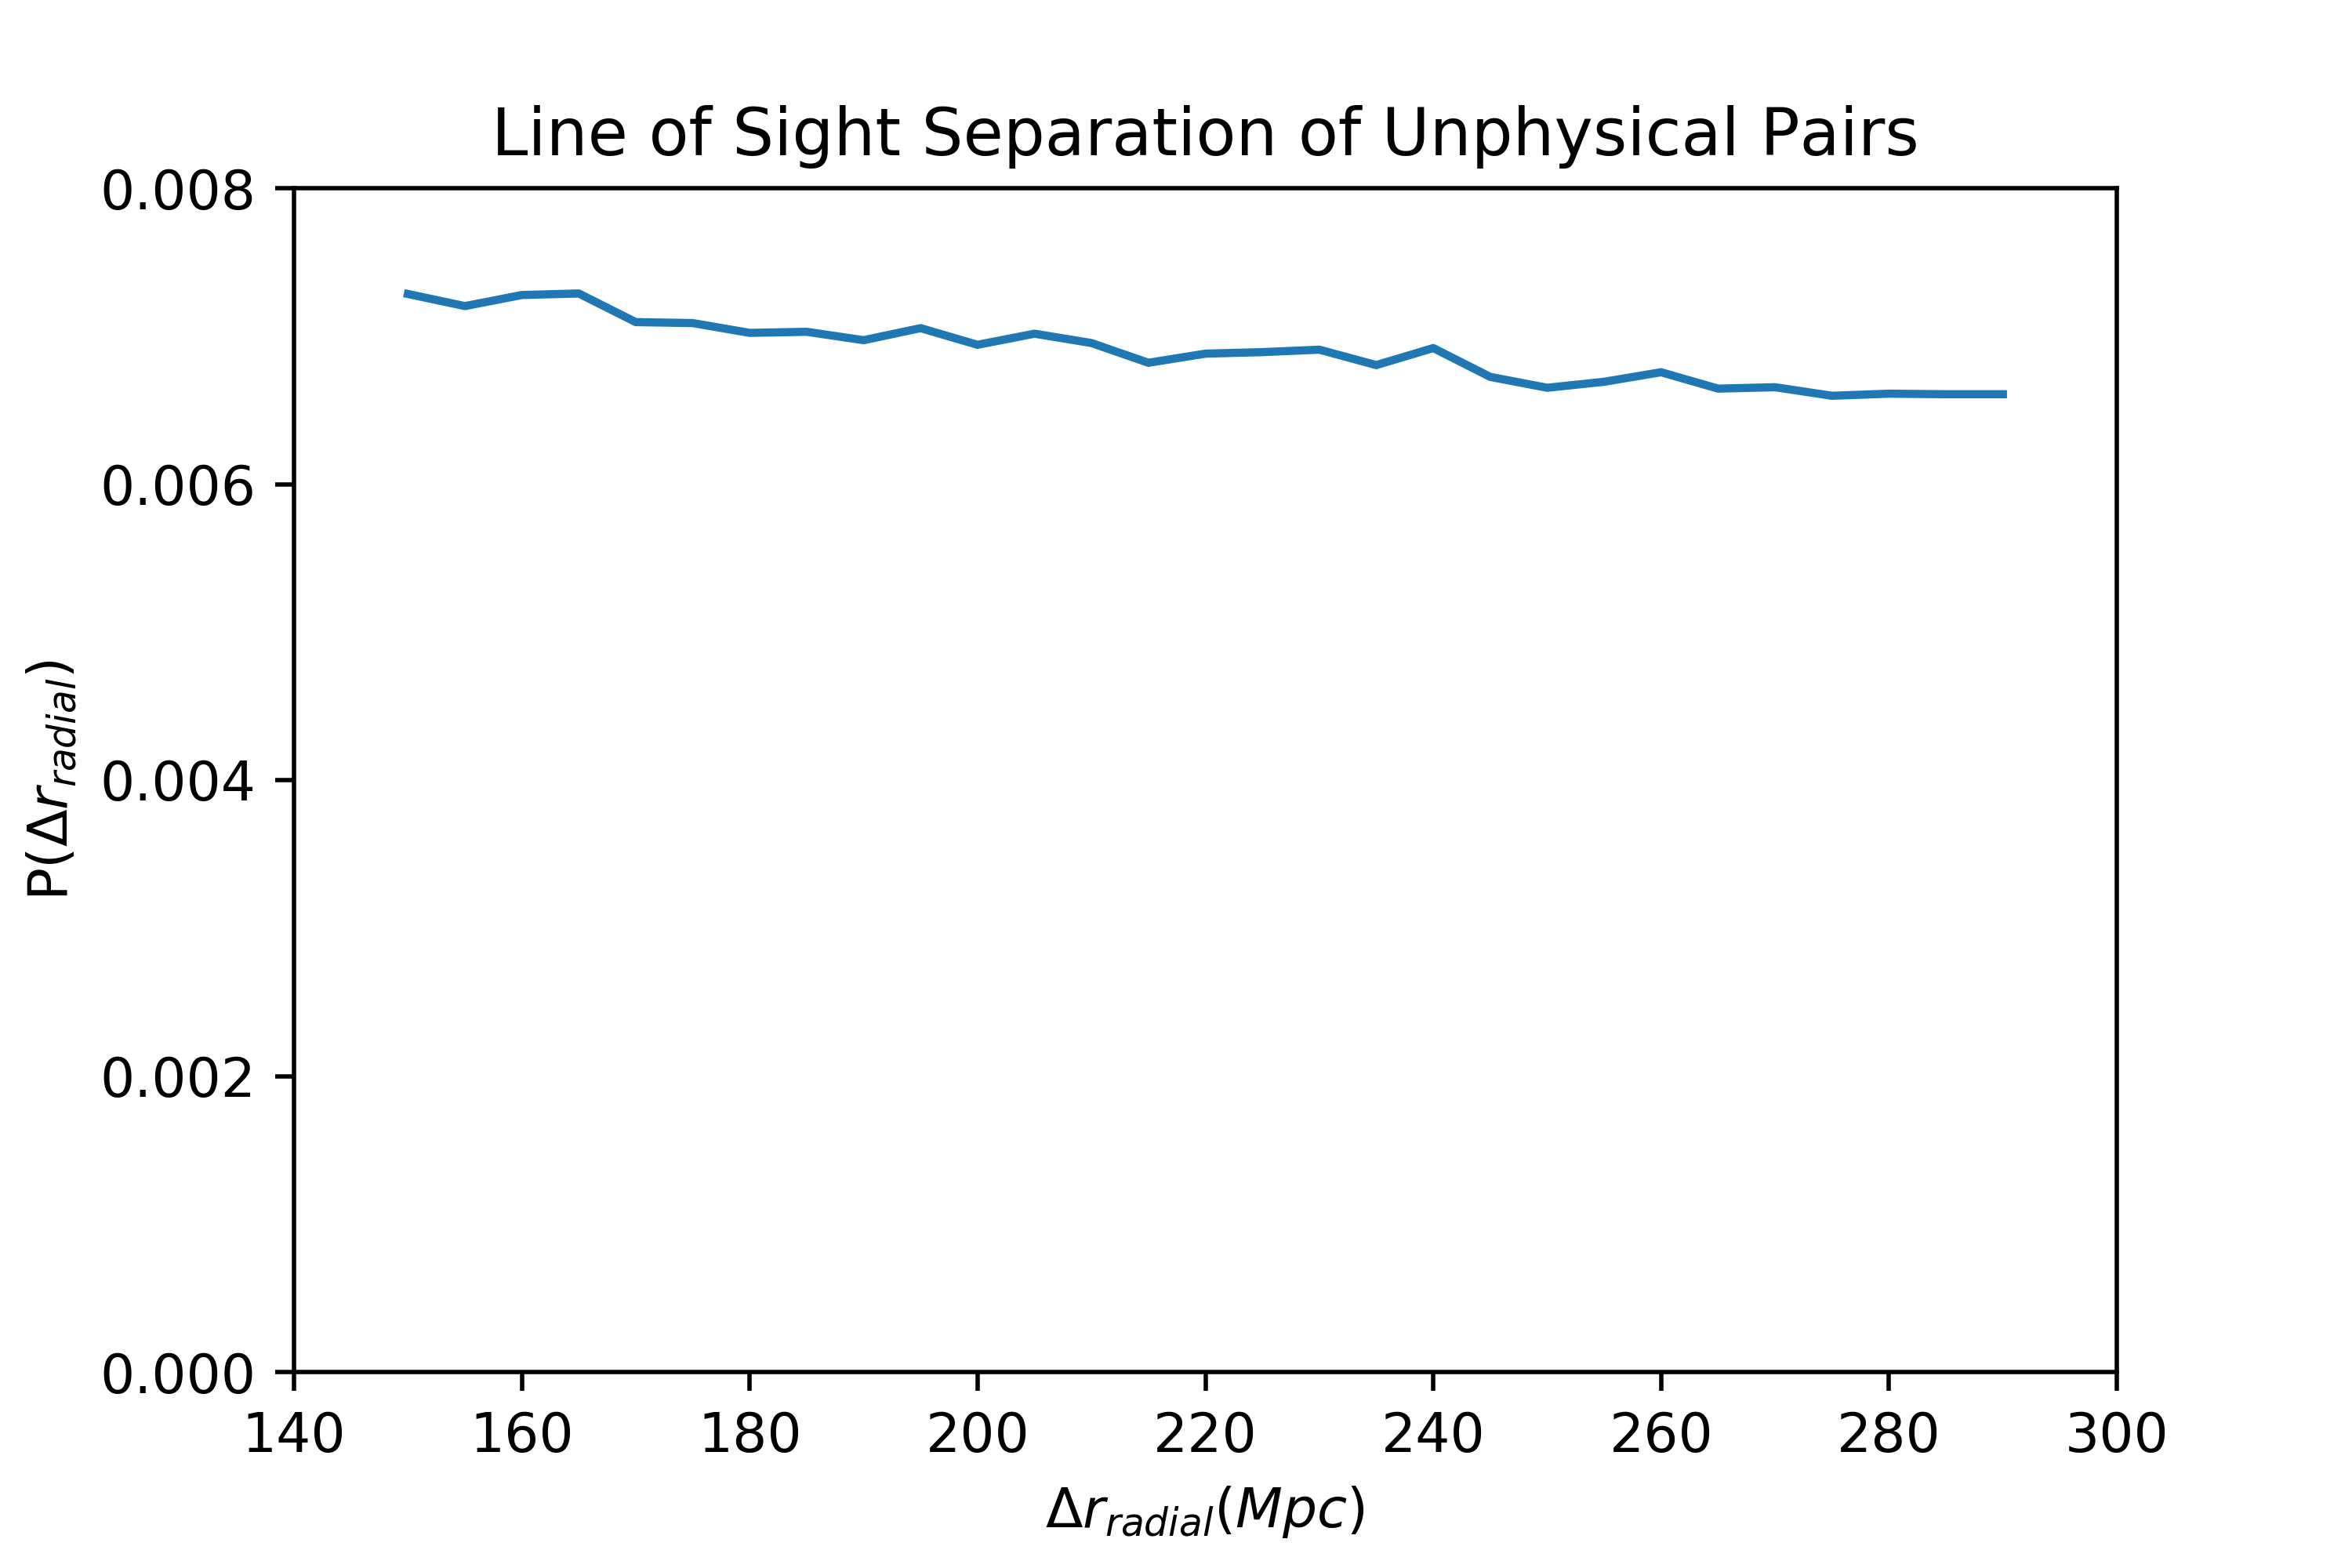
\includegraphics[width=0.6\textwidth, keepaspectratio]{/home/mitchell/Documents/masters/masters/thesis/Ver_2/figures/UP_LOS_Separation.png}
\caption{Histogram of Line of Sight Separations of Unphysical Galaxy Pairs. The distribution is relatively flat, with the same shape as the physical pairs, a minimum separation of $\SI{147}{\mega\parsec}$, and a maximum separation of $\SI{295}{\mega\parsec}$.  }
\label{fig:unphysical:lineofsight}
\end{figure}

The choice was made to consider unphysical pairs with a line of sight separation in excess of $\SI{100}{\per\h\mega\parsec}$ because at large redshifts, the errors assosciated with the photometric redshifts can place a very large range on the possible distance to a given galaxy, and we want to be very careful to exclude galaxy pairs that might have a connecting filament between them. 

\begin{figure}[H]
\centering
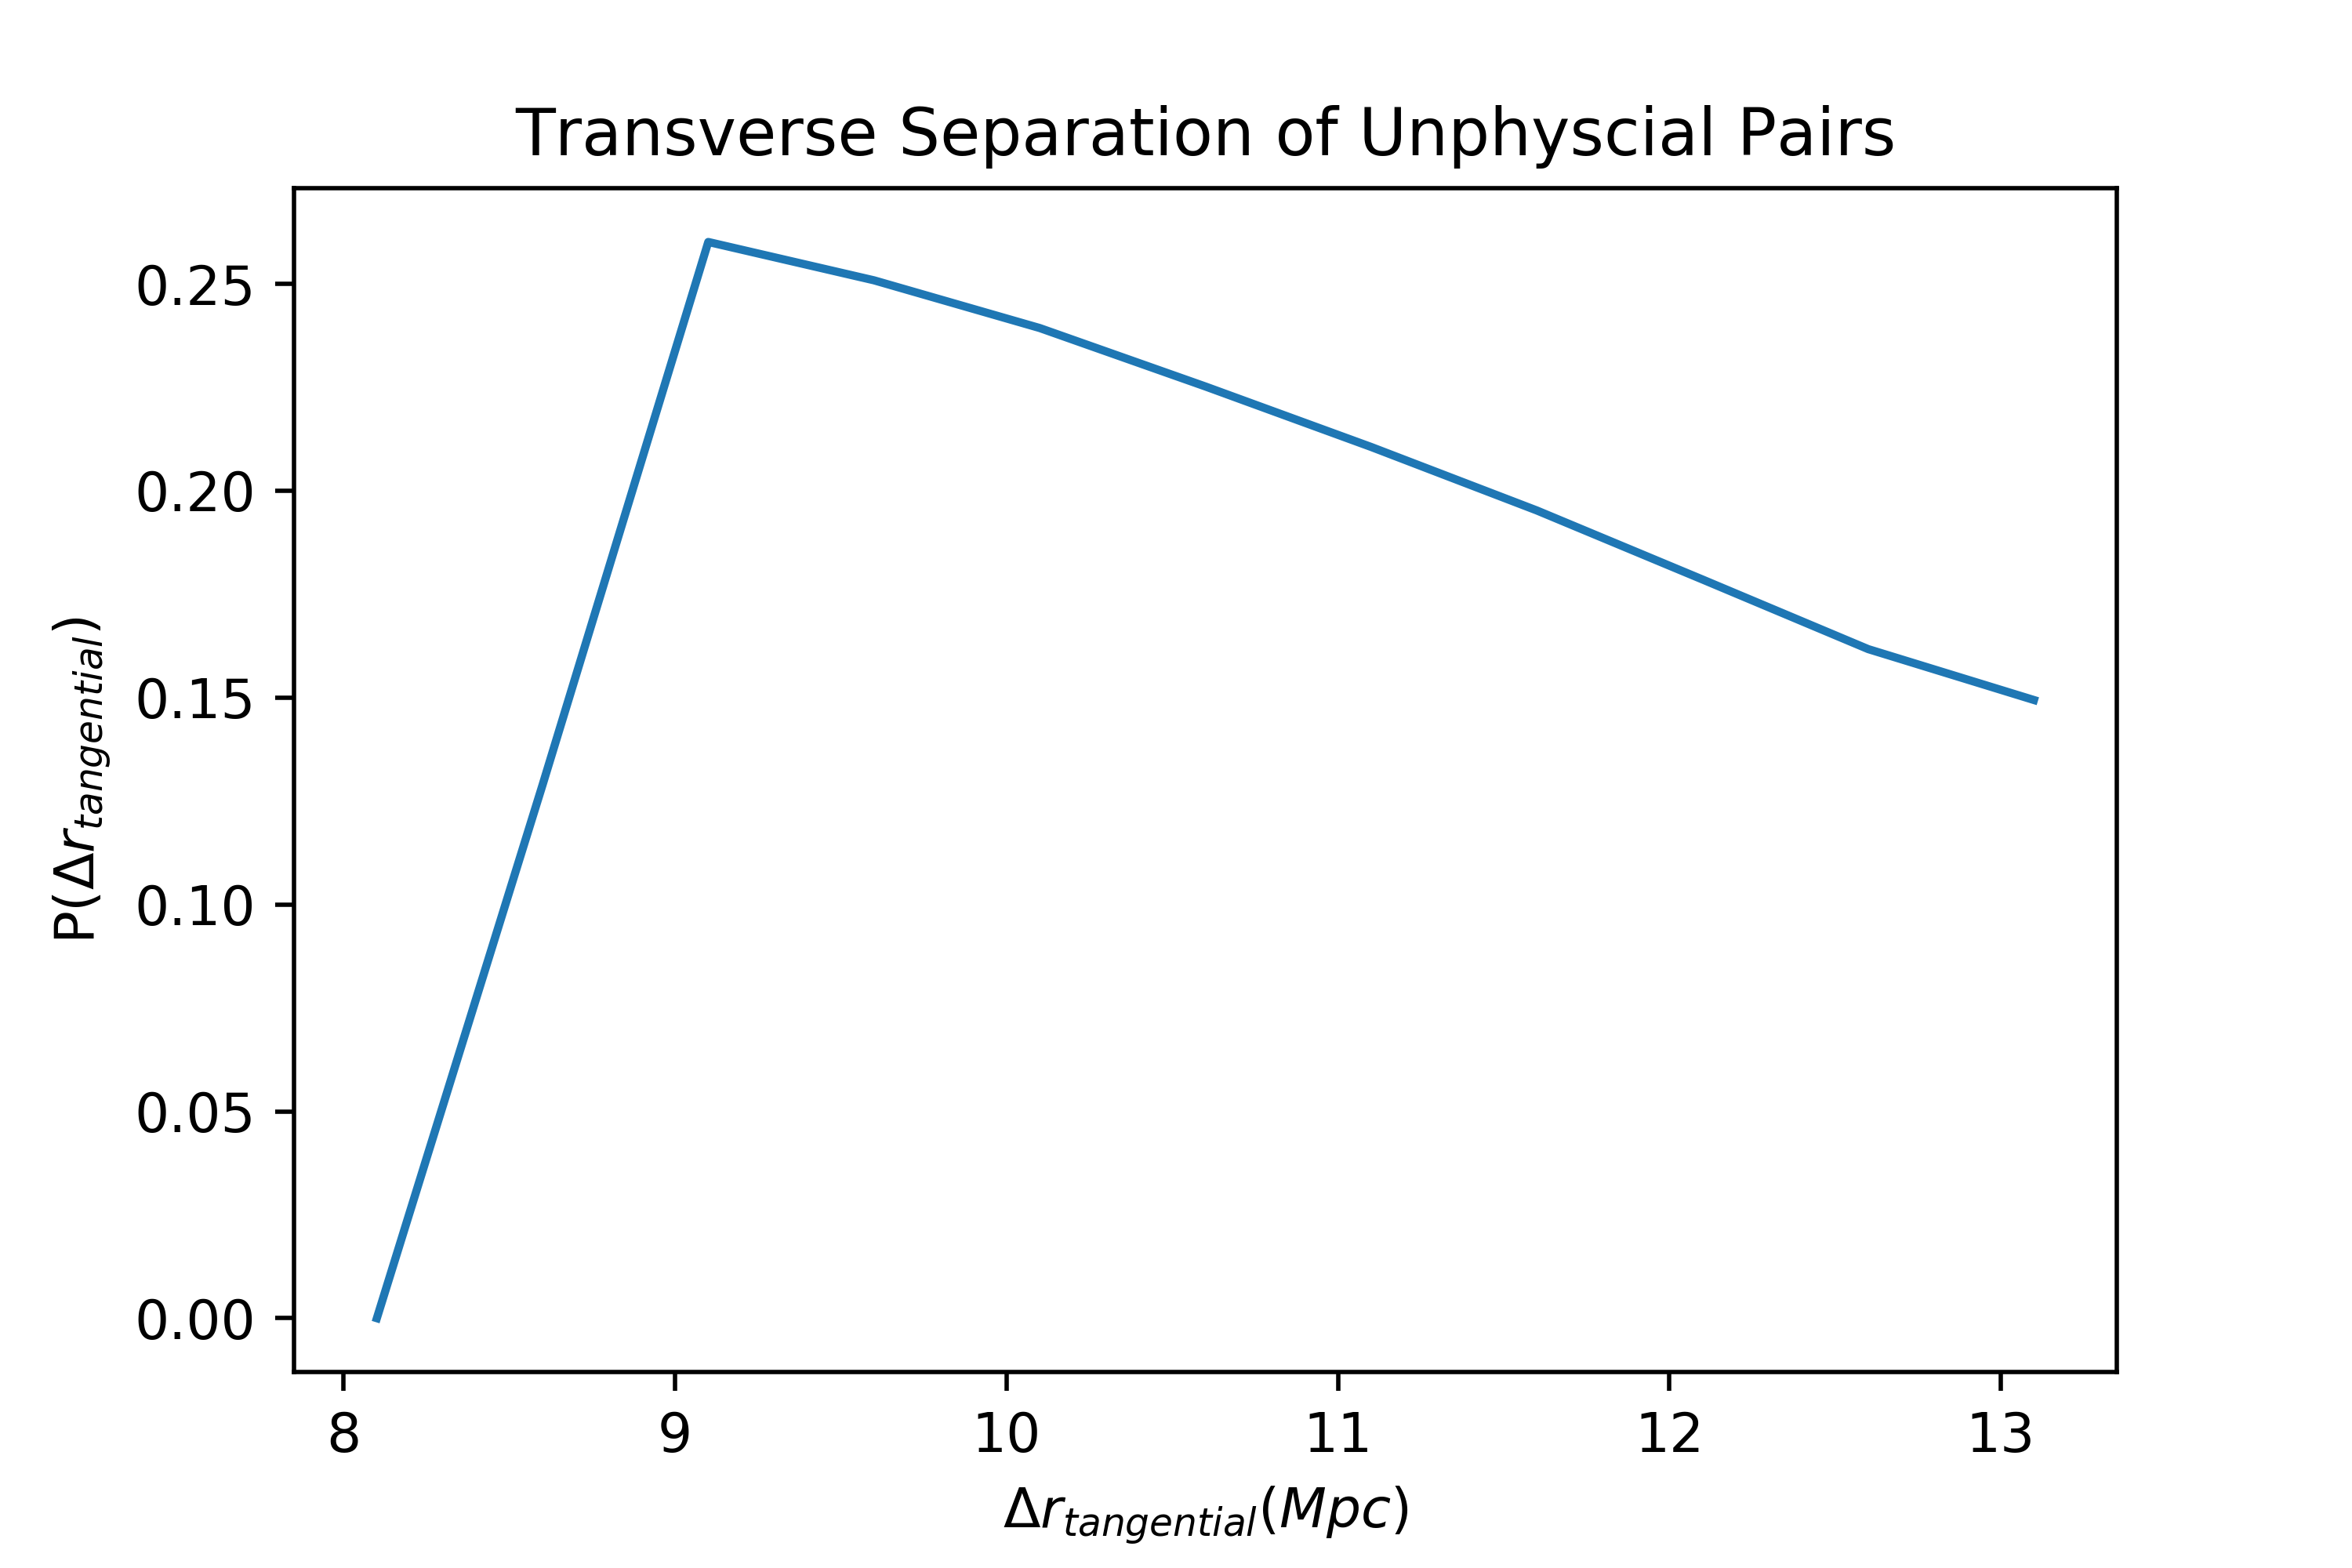
\includegraphics[width=0.6\textwidth  , keepaspectratio]{/home/mitchell/Documents/masters/masters/thesis/Ver_2/figures/UP_TRV_Separation.png}
\caption{Histogram of Transverse Separations of Unphysical Galaxy Pairs. The distribution is relatively flat, with a minimum seperation of $\SI{8.85}{\mega\parsec}$ and a maximum separation $\SI{20.7}{\mega\parsec}$. This has the same overall shape as the physical pairs data set, except the relative population in the higher separation bins decreases, rather than increases.}
\label{fig:unphysical:transverse}
\end{figure}

Performing the stacking procedure on the unphysical dataset gives the stack shown in figure \ref{fig:unphysical:stack}. To the eye, in both the 2D slice and the 3D colour map, it appears that there is less filamentary signal than for the physical pairs. 

\begin{figure}[H]
\centering
\includegraphics[width=0.8\textwidth , keepaspectratio]{/home/mitchell/Documents/masters/masters/thesis/Ver_2/figures/UnPhysical_Stack.png}
\caption{Stacked Image of Unphyiscal pairs.}
\label{fig:unphysical:stack}
\end{figure}

If we fit the two halos for gaussian profiles (shown in figure \ref{fig:halo:basic_filament}) , along with some constant offset, we can see very clearly that there appears to be no residual signal left. The mean of this residual is $3.48 \times 10^{-18}$, with a variance of $1.13 \times 10^{-16}$, which is consistent with a zero measurement. 


\begin{figure}[H]
\centering
\includegraphics[width=\textwidth , keepaspectratio]{/home/mitchell/Documents/masters/masters/thesis/Ver_2/figures/unphysical_halo_fit.png}
\caption{Gaussian Fit to Unphysical Pairs}
\label{fig:unphysical:fit}
\end{figure}

\subsection{Random Stack}

Performing a stack on a set of pseudo-randomly selected slices of the CMB, with the same galactic latitude as the physical pairs, we produced a stack like the one shown in Figure \ref{fig:random:stack}. This has no discernable structure, except for the small circular signal in the centre of the map. This is likely due to the rescaling effect still rescaling the CMB as if it were trying to align pairs. Because the angle that the pairs need to be rotated by should be evenly distributed, there should be some level of correlation in the stack, in a circular structure where we would otherwise expect a filament to be. 

\begin{figure}[H]
\centering
\includegraphics[width=\textwidth , keepaspectratio]{/home/mitchell/Documents/masters/masters/thesis/Ver_2/figures/Rand_Pos_Stack.png}
\caption{Stack of pseudo-random slices}
\label{fig:random:stack}
\end{figure}

